\chapter[One-Dimensional Bloch-to-Lattice Reduction]{From Bloch Fibers to Finite-Range Lattice Hamiltonians in a One-Dimensional Cosine Potential}
\index{warmup!one-dimensional|textbf}

\label{app:one-dimensional-reduction}

\chapterstatus{calculated illustrative numerical verification. Independent
discretizations, isolated- and composite-band reductions, and a converged
Wannier90 comparison establish the numerical behavior of the specified cosine
model. The results do not constitute semiconductor validation or evidence of
transferability to silicon.}

\section*{Abstract}

Reducing a periodic continuum Hamiltonian to a finite-range lattice model
requires controlled choices of representation, retained subspace, gauge, and
truncation. We examine these choices in a one-dimensional cosine lattice using
independently refined plane-wave and finite-difference discretizations. For the
isolated lowest band, localized hopping reconstruction reproduces the parent
dispersion, withheld errors decrease with hopping range, and direct Fourier
fitting agrees with truncation of the localized operator. Stress tests show that
scalar-band tracking becomes unreliable near gap closures and for poorly
conditioned higher bands. Composite-band transport resolves this label
instability, while controlled gauge perturbations demonstrate that finite-range
locality is not gauge invariant. An independent Wannier90 localization implementation applied
to the same spectral and overlap data converges with preconditioning and
reproduces the direct centers and common-frame operators to the reported
numerical accuracy.

\section{Introduction}

Localized lattice Hamiltonians mediate between periodic continuum operators and
the reduced models used in solid-state and semiconductor physics. Wannier's
original construction introduced localized orbitals for periodic systems, and
subsequent work established their analytic localization properties and the
modern variational treatment of isolated and composite band manifolds
\cite{wannier1937,kohn1959,marzari1997,souza2001,marzari2012}. Contemporary
implementations make these constructions available for realistic electronic
structure calculations~\cite{pizzi2020}.

The passage from a continuum operator to a finite-range model is nevertheless
not determined by band energies alone. It also requires a retained state space,
a reciprocal-space gauge, a localization convention, and a real-space
truncation. Each choice introduces a distinct approximation or coordinate
dependence. Comparing final spectra without controlling these intermediate
objects can therefore conceal representation errors, subspace mismatch, or
compensating fit errors.

The cosine lattice considered here isolates those issues in a problem whose
Bloch fibers, Fourier couplings, reciprocal sewing, and hopping transform can be
inspected directly. It supplies a controlled analogue of two reduction routes:
\begin{align}
    \text{periodic parent}
    &\longrightarrow
    \text{finite-range lattice model},
    \label{eq:periodic-1d-direct-route}
    \\
    \text{periodic parent}
    &\longrightarrow
    \text{localized represented operator}
    \longrightarrow
    \text{finite-range lattice model}.
    \label{eq:periodic-1d-mediated-route}
\end{align}
The first route fits a specified Fourier class directly to reciprocal-space
data. The second constructs the complete represented hopping operator and then
truncates it in real space. Under matched grids, weights, coordinates, and model
classes, the two routes are the same orthogonal projection. Controlled changes
to those conditions expose when and why they cease to agree.

The study addresses four related questions. First, do independent
plane-wave and finite-difference representations converge to the same parent
operator after transport into common coordinates? Second, when is an individual
band sufficiently isolated for scalar parallel transport and Wannier
construction? Third, can a composite retained subspace replace unstable
energy-ordered band labels while preserving a comparable represented operator?
Fourth, how do gauge choice and hopping range affect the accuracy of the final
lattice model? A separate Wannier90 calculation tests the localization
interface and implementation without introducing an independent physical
parent. The contribution is not a new localization algorithm; it is a
controlled benchmark that places discretization error, subspace conditioning,
gauge covariance, finite-range truncation, and route equivalence in one
quantitative setting.

\section{Continuum parent and exact structure}

Let the lattice period be $a$, define $G=2\pi/a$, and consider
\begin{equation}
    \hat H
    =
    -\frac{\hbar^2}{2m}\frac{d^2}{dx^2}
    +V_0\cos(Gx)
    \quad\text{on }L^2(\mathbb R).
    \label{eq:periodic-1d-parent}
\end{equation}
The natural reciprocal energy scale is
\begin{equation}
    E_G=\frac{\hbar^2G^2}{2m},
    \qquad
    \lambda=\frac{V_0}{E_G}.
    \label{eq:periodic-1d-scales}
\end{equation}
Bloch states have the form
\begin{equation}
    \psi_{nk}(x)=e^{ikx}u_{nk}(x),
    \qquad
    u_{nk}(x+a)=u_{nk}(x),
\end{equation}
and the cell-periodic fiber operator is
\begin{equation}
    \hat H(k)
    =
    \frac{1}{2m}
    \left(-i\hbar\frac{d}{dx}+\hbar k\right)^2
    +V_0\cos(Gx).
    \label{eq:periodic-1d-fiber}
\end{equation}
Equivalently, the original differential expression can act on a single cell
with Bloch boundary conditions
\begin{align}
    \psi(a)&=e^{ika}\psi(0),
    &
    \psi'(a)&=e^{ika}\psi'(0).
\end{align}
These two conventions are unitarily related, but their matrices must not be
mixed without an explicit transformation.

The real inversion-symmetric parent obeys
\begin{align}
    E_n(k+G)&=E_n(k),
    &
    E_n(-k)&=E_n(k),
    \label{eq:periodic-1d-symmetry}
\end{align}
after consistent band matching. The sign change $V_0\mapsto -V_0$ translates
the potential by $a/2$ and leaves the spectrum invariant. In the weak-potential
regime, the Fourier coefficient $V_0/2$ couples crossing free-particle states
and gives a leading first-zone-boundary gap of $|V_0|$. These identities provide
structural and perturbative checks that are independent of either numerical
representation.

With $z=Gx/2$, Eq.~\eqref{eq:periodic-1d-parent} becomes the Mathieu equation
\begin{equation}
    \frac{d^2\psi}{dz^2}
    +\left[A-2q\cos(2z)\right]\psi=0,
    \qquad
    A=\frac{4E}{E_G},
    \quad
    q=\frac{2V_0}{E_G},
    \label{eq:periodic-1d-mathieu}
\end{equation}
with Floquet condition
\begin{equation}
    \psi(z+\pi)=e^{ika}\psi(z),
    \qquad
    \nu=\frac{2k}{G}\pmod 2.
\end{equation}
For the chosen Brillouin zone, $-1\leq\nu<1$; the equivalent representatives
$0\leq\nu<2$ follow by reduction modulo 2. The checks used below are restricted
to branches whose indexing is unambiguous: the lowest zone-center energy is
$a_0(q)E_G/4$, while the two lowest zone-boundary energies are the sorted values
$a_1(q)E_G/4$ and $b_1(q)E_G/4$. These characteristic values provide a
reference that does not reuse either matrix discretization; the notation and
Floquet convention follow the standard Mathieu-function
treatment~\cite{mclachlan1947}.

\section{Numerical representations of the parent}

\subsection{Plane-wave Galerkin representation}

In the Bloch plane-wave basis
\begin{equation}
    \langle x\mid n,k\rangle
    =
    \frac{1}{\sqrt a}e^{i(k+nG)x},
    \qquad n\in\mathbb Z,
\end{equation}
the fiber matrix is
\begin{equation}
    H^{\mathrm{PW}}_{nm}(k)
    =
    \frac{\hbar^2(k+nG)^2}{2m}\delta_{nm}
    +\frac{V_0}{2}
    \left(\delta_{n,m+1}+\delta_{n,m-1}\right).
    \label{eq:periodic-1d-pw-matrix}
\end{equation}
The nearest-neighbor structure in reciprocal index is an exact consequence of
the potential's Fourier content, not a real-space tight-binding approximation.
A cutoff $P$ retains $n=-P,\ldots,P$ and defines the Galerkin matrix
$\mathbf H_P^{\mathrm{PW}}(k)\in\mathbb C^{(2P+1)\times(2P+1)}$.
At fixed $k$, the largest represented free-particle energy is
$E_G\max_{|n|\leq P}(k/G+n)^2$; its supremum over the first Brillouin zone is
$(P+1/2)^2E_G$. Convergence of low bands must be distinguished from the behavior
of states near this reciprocal cutoff.

\subsection{Finite-difference Bloch-boundary representation}

A second representation acts on one unit cell with
\begin{equation}
    x_j=j\Delta x,
    \qquad
    \Delta x=\frac{a}{N},
    \qquad
    j=0,\ldots,N-1.
\end{equation}
For the centered second-order kinetic stencil, let
\begin{equation}
    t_h=\frac{\hbar^2}{2m\Delta x^2}.
\end{equation}
The kinetic matrix has diagonal entries $2t_h$, nearest-neighbor entries
$-t_h$, and boundary entries
\begin{align}
    T^{\mathrm{FD}}_{0,N-1}(k)&=-t_h e^{-ika},
    &
    T^{\mathrm{FD}}_{N-1,0}(k)&=-t_h e^{ika}.
\end{align}
Together with
\begin{equation}
    \mathbf V_h
    =
    \operatorname{diag}\left(V_0\cos(Gx_0),\ldots,V_0\cos(Gx_{N-1})\right),
\end{equation}
this gives
\begin{equation}
    \mathbf H_h^{\mathrm{FD}}(k)
    =\mathbf T_h^{\mathrm{FD}}(k)+\mathbf V_h.
    \label{eq:periodic-1d-fd-matrix}
\end{equation}
Hermiticity requires conjugate boundary phases. A failure of this condition is
an implementation error rather than a physical band effect.

For a discrete Bloch wave with $q=k+nG$, the represented kinetic energy is
\begin{equation}
    \varepsilon_h^{\mathrm{kin}}(q)
    =
    \frac{2\hbar^2}{m\Delta x^2}
    \sin^2\left(\frac{q\Delta x}{2}\right)
    =
    \frac{\hbar^2q^2}{2m}
    \left[1-\frac{(q\Delta x)^2}{12}
    +O\!\left((q\Delta x)^4\right)\right].
    \label{eq:periodic-1d-fd-dispersion}
\end{equation}
The expected second-order error applies to fixed smooth modes, not to modes
approaching the grid cutoff.

\subsection{Comparison in common coordinates}

Matrices of different dimensions or in different bases cannot be subtracted
directly. Choosing $N=2P+1$ gives equal matrix dimensions, after which the
discrete Bloch--Fourier matrix
\begin{equation}
    F_{jn}(k)
    =\frac{1}{\sqrt N}e^{i(k+nG)x_j},
    \qquad n=-P,\ldots,P,
\end{equation}
transports the finite-difference matrix into discrete plane-wave coordinates:
\begin{equation}
    \mathbf A_h^{\mathrm{FD}\rightarrow\mathrm{PW}}(k)
    =
    \mathbf F(k)^\dagger
    \mathbf H_h^{\mathrm{FD}}(k)
    \mathbf F(k).
\end{equation}
The full common-coordinate discrepancy is
\begin{equation}
    D_{\mathrm{rep}}(k;h,P)
    =
    \left\lVert
        \mathbf A_h^{\mathrm{FD}\rightarrow\mathrm{PW}}(k)
        -\mathbf H_P^{\mathrm{PW}}(k)
    \right\rVert_{\mathrm F}.
\end{equation}
Because cutoff modes can dominate this norm, a fixed low-mode sector is also
used. If $\mathbf P_L$ selects $|n|\leq L<P$, then
\begin{equation}
    D_{\mathrm{rep}}^{(L)}(k;h,P)
    =
    \left\lVert
        \mathbf P_L
        \left(
            \mathbf A_h^{\mathrm{FD}\rightarrow\mathrm{PW}}(k)
            -\mathbf H_P^{\mathrm{PW}}(k)
        \right)
        \mathbf P_L
    \right\rVert_{\mathrm F}.
    \label{eq:periodic-1d-common-discrepancy}
\end{equation}
The sampled potential may wrap Fourier couplings across the finite cyclic grid.
Discrete Fourier indices are identified modulo $N$, so on a coarse grid the
$\pm G$ harmonic can connect the endpoint reciprocal indices through cyclic
wraparound. That aliasing is a property of the representation and must not be
interpreted as a physical long-range Fourier component.

\section{Retained subspaces and localization}

\subsection{Isolation and subspace diagnostics}

Let $E_n(k)$ denote ordered fiber eigenvalues. An individual band is treated as
isolated only when its separation from neighboring bands remains above the
prescribed threshold over the complete reciprocal mesh. Near close approaches,
independent energy sorting is insufficient: it can exchange labels while
leaving the combined subspace continuous.

For two retained frames represented in common ambient coordinates,
$\mathbf B_1(k)$ and $\mathbf B_2(k)$, define
\begin{equation}
    \mathbf S(k)=\mathbf B_1(k)^\dagger\mathbf B_2(k).
\end{equation}
The singular values of $\mathbf S(k)$ measure neighboring or cross-representation
subspace compatibility. The associated projector discrepancy is
\begin{equation}
    D_P(k)
    =
    \left\lVert
        \mathbf B_1(k)\mathbf B_1(k)^\dagger
        -\mathbf B_2(k)\mathbf B_2(k)^\dagger
    \right\rVert_{\mathrm F}.
\end{equation}
Because the Frobenius norm is definite, $D_P(k)=0$ if and only if the two
orthogonal projectors are identical. Spectral agreement, subspace agreement,
and basis agreement are therefore reported separately.

\subsection{Isolated-band parallel transport}

For normalized cell-periodic states at neighboring mesh points, define
\begin{equation}
    m_j=\langle u_{k_j}\mid u_{k_{j+1}}\rangle.
\end{equation}
When $m_j\neq0$, the phase of $u_{k_{j+1}}$ is chosen so that $m_j$ is real and
nonnegative. Sequential transport gives a smooth frame, while reciprocal sewing
at the Brillouin-zone boundary supplies a closure holonomy. Distributing that
phase over the mesh produces a periodic gauge. A small $|m_j|$ instead signals poor matching, insufficient sampling, or
failure of the isolated-band model; phase smoothing cannot repair the loss of
a retained subspace. No universal overlap threshold is imposed here. Overlap
magnitudes are interpreted together with gap closure and reciprocal-mesh
refinement rather than converted into an automatic scalar-to-composite switch.

For a uniform $N_k$-point mesh and Born--von Karman representatives
$R\in\mathcal R_{N_k}$, the Wannier states are
\begin{equation}
    \lvert w_R\rangle
    =
    \frac{1}{\sqrt{N_k}}
    \sum_k e^{-ikR}\lvert\psi_k\rangle.
    \label{eq:periodic-1d-wannier-transform}
\end{equation}
A smooth periodic phase changes the Wannier profile but preserves the center
modulo $a$. A reciprocal winding translates its representative by a lattice
vector. The isolated-band projector and scalar dispersion remain invariant
under either compatible gauge change~\cite{kohn1959,marzari2012}.

\subsection{Composite-band transport}

For an $M$-band retained space, the neighboring overlap matrix is
\begin{equation}
    \mathbf M^{(j)}_{mn}
    =\langle u_{m,k_j}\mid u_{n,k_{j+1}}\rangle.
    \label{eq:periodic-1d-neighbor-overlap}
\end{equation}
Its singular values distinguish a change of frame from a loss of subspace
overlap. The unitary polar factor supplies the orthogonal-Procrustes rotation
that maximizes neighboring-frame overlap~\cite{schonemann1966}. Sequential
polar transport and reciprocal closure define a smooth composite frame and a
Wilson-loop matrix. The Wilson eigenphases give hybrid Wannier centers modulo
lattice translations, consistent with the composite-band framework of
Refs.~\cite{marzari1997,souza2001}.

A momentum-dependent unitary transformation changes the frame, individual
Wannier functions, and real-space matrix blocks but leaves the retained
projector invariant. Pointwise operator subtraction is meaningful only after
both frames have been transformed into common coordinates. In this study the
required alignment is obtained from the unitary polar factor of the frame
overlap at each reciprocal point.

\subsection{Wannier90 interface}

Wannier90 provides an independent implementation of localization, not an
independent parent calculation. It consumes eigenvalues, neighboring-state
overlaps
\begin{equation}
    M_{mn}^{(\mathbf k,\mathbf b)}
    =
    \langle u_{m\mathbf k}\mid u_{n,\mathbf k+\mathbf b}\rangle,
\end{equation}
and trial projections
\begin{equation}
    A_{mn}(\mathbf k)
    =\langle\psi_{m\mathbf k}\mid g_n\rangle.
\end{equation}
The standard file interface represents these quantities through
\texttt{.eig}, \texttt{.mmn}, \texttt{.amn}, and \texttt{.win} files. The
overlap matrices must use cell-periodic states, the specified inner product, and
consistent reciprocal-boundary relabelling; energies alone cannot define the
localization problem~\cite{souza2001,pizzi2020}.

The one-dimensional parent is embedded in a $128\times1\times1$ reciprocal
mesh with an auxiliary transverse cell and a unit transverse form factor. Those
inactive directions are representation conventions, not physical dimensions
of the parent. The comparison retains two bands and two Wannier functions per group, identity
projections in the retained eigenbasis,
\texttt{search\_shells = 130}, \texttt{num\_iter = 5000},
\texttt{conv\_tol} $=10^{-12}$, a five-iteration convergence window, and
\texttt{precond = true}. Direct and Wannier90 outputs are compared only after
orbital order, lattice translations, and composite-space unitary freedom have
been aligned.

\section{Finite-range lattice reduction}

\subsection{Complete hopping representation}

For one isolated band, the complete represented hopping coefficients are
\begin{equation}
    t(R)
    =
    \langle w_0\rvert\hat H\lvert w_R\rangle
    =
    \frac{1}{N_k}\sum_k e^{-ikR}E(k),
    \qquad R\in\mathcal R_{N_k},
    \label{eq:periodic-1d-scalar-hopping}
\end{equation}
with inverse transform
\begin{equation}
    E(k)=\sum_{R\in\mathcal R_{N_k}}e^{ikR}t(R).
\end{equation}
For a composite group, the corresponding matrix blocks are
\begin{equation}
    \mathbf H_{\mathrm W}(R)
    =
    \frac{1}{N_k}\sum_k
    e^{-ikR}\mathbf H_{\mathrm W}(k).
    \label{eq:periodic-1d-block-hopping}
\end{equation}
The complete scalar transform depends only on the represented band dispersion.
For the present time-reversal- and inversion-symmetric scalar band, $E(k)$ is
real and even, so the exact transform gives real $t(R)=t(-R)$; the residual
imaginary components below measure numerical error. Composite blocks
additionally depend on the selected frame.

\subsection{Finite hopping range}

For a symmetric retained set $\mathcal R_c\subset\mathcal R_{N_k}$, define
\begin{align}
    E_{\mathrm{TB}}^{(\mathcal R_c)}(k)
    &=
    \sum_{R\in\mathcal R_c}e^{ikR}t(R),
    \\
    \mathbf H_{\mathrm{TB}}^{(\mathcal R_c)}(k)
    &=
    \sum_{R\in\mathcal R_c}e^{ikR}\mathbf H_{\mathrm W}(R).
\end{align}
Hermiticity requires $t(-R)=t(R)^\ast$ and
$\mathbf H_{\mathrm W}(-R)=\mathbf H_{\mathrm W}(R)^\dagger$ under the chosen
Born--von Karman representative convention. The scalar residual is
\begin{equation}
    \Delta E^{(\mathcal R_c)}(k)
    =
    \sum_{R\notin\mathcal R_c}e^{ikR}t(R).
\end{equation}
On the complete uniform transform, Parseval's identity gives
\begin{equation}
    \sum_k\left|\Delta E^{(\mathcal R_c)}(k)\right|^2
    =
    N_k\sum_{R\notin\mathcal R_c}|t(R)|^2.
    \label{eq:periodic-1d-parseval}
\end{equation}
Thus reciprocal residuals and omitted hopping norms are equivalent descriptions
only under the stated finite-transform conventions. In particular, decreasing
the omitted hopping norm decreases the mean-square reciprocal-space error on
the complete training mesh. For composite bands the same construction applies
to Frobenius norms of the aligned matrix residuals.

The lattice model approximates a retained Bloch operator or its dispersion. It
does not converge directly to the scalar multiplication potential. Recovering a
potential from reduced spectral or hopping data is a different inverse problem.

\subsection{Direct and mediated routes}

For an isolated band, a weighted direct Fourier fit minimizes
\begin{equation}
    \mathcal L_{\mathrm{dir}}(\{t(R)\})
    =
    \sum_{k\in\mathcal T}w_k
    \left|
        E_{\mathrm{parent}}(k)
        -\sum_{R\in\mathcal R_c}e^{ikR}t(R)
    \right|^2.
    \label{eq:periodic-1d-direct-objective}
\end{equation}
The mediated route first evaluates Eq.~\eqref{eq:periodic-1d-scalar-hopping} on
the complete mesh and then discards blocks outside $\mathcal R_c$. With a
complete uniform mesh, equal weights, compatible transforms, and the same
unconstrained Hermitian Fourier class, both procedures are the same orthogonal
projection. They need not agree for nonuniform weights, restricted training
domains, parameter-sharing constraints, different gauges, incompatible grids,
or different objective observables.

For aligned final matrix models, define the \emph{route defect}
\begin{equation}
    D_{\mathrm{path}}^2
    =
    \sum_{k\in\mathcal K_{\mathrm{cmp}}}w_k
    \left\lVert
        \mathbf H_{\mathrm{TB,dir}}(k)
        -\mathbf H_{\mathrm{TB,med}}(k)
    \right\rVert_{\mathrm F}^2.
    \label{eq:periodic-1d-path-defect}
\end{equation}
The route defect separates a change of reduction route from a change of fitting
problem.

\section{Numerical protocol}

The nominal isolated-band calculation uses the dimensionless convention
$a=2\pi$, $G=1$, and $E_G=1$, with $V_0/E_G=0.5$. Plane-wave cutoffs
$P=3,5,7,9,11$ are compared with a $P=15$ reference. The corresponding
Brillouin-zone supremum kinetic cutoffs are obtained from
$(P+1/2)^2E_G$. The finite-difference study uses $N=31,63,127,255$ cell points,
with exact spacings $\Delta x/a=1/N$. Parent comparisons are made at
$k/G=-0.5,-0.25,0,0.25,0.5$ in the fixed low-mode sector $|n|\leq3$.
The isolated-band hopping transform uses 64 reciprocal points, ranges
$r_c/a=0,1,2,3,4,6,8$, and an independent 257-point withheld mesh.

The sensitivity analysis spans $V_0/E_G=0,0.02,0.1,0.5,1,2,4$, reciprocal
meshes from 8 to 128 points, and the first eight bands. A $P=21$ plane-wave
calculation is the higher-band reference. Translated, constant-shifted,
second-harmonic, inversion-breaking, and three-harmonic real potentials test
symmetry and model dependence. Random phase perturbations test gauge covariance,
while nonuniform weights and restricted training regions change the direct
fitting objective one condition at a time.

The composite calculation uses $P=15$, a 128-point reciprocal mesh, a 257-point
withheld mesh, and band groups 0--1 and 2--3. Hopping ranges extend to
$r_c=12a$. The external-gap threshold is $10^{-8}E_G$. Controlled smooth and
rough $U(2)$ transformations test covariance and locality. Equal-weight direct
and mediated matrix reductions are compared at $r_c=4a$.

The analysis reports the following error sources separately:
\begin{enumerate}
    \item plane-wave cutoff error;
    \item finite-difference grid and stencil error;
    \item Bloch-boundary and structural residuals;
    \item reciprocal sampling and Fourier-transform error;
    \item retained-band or retained-subspace conditioning;
    \item overlap, reciprocal-sewing, and localization error;
    \item gauge and alignment sensitivity;
    \item hopping-range truncation error;
    \item direct-fit objective and route discrepancy;
    \item serialized-Hamiltonian precision; and
    \item observable-extraction error.
\end{enumerate}
No combined uncertainty is formed because no mathematical relation among these
error classes has been established.

\section{Results}

\subsection{Parent representation verification}

The plane-wave and finite-difference sequences converge independently.
Table~\ref{tab:periodic-1d-parent-convergence} reports representative endpoint
errors. For the lowest three bands, the plane-wave error relative to $P=15$
decreases by more than seven orders of magnitude between $P=3$ and $P=5$. The
finite-difference sequence exhibits the slower convergence expected from the
second-order dispersion error in
Eq.~\eqref{eq:periodic-1d-fd-dispersion}. Selected plane-wave energies agree
with independently evaluated Mathieu characteristic values within
$1.2\times10^{-16}E_G$.

\begin{table}[htbp]
  \centering
  \caption{Representative parent-discretization errors in units of $E_G$.
  Spectral errors are maxima over the lowest three bands and the sampled
  momenta. The common-coordinate discrepancy is the Frobenius norm in the fixed
  $|n|\leq3$ sector.}
  \label{tab:periodic-1d-parent-convergence}
  \small
  \begin{tabular}{lrr}
    \toprule
    Quantity & Coarse & Fine \\
    \midrule
    Plane-wave spectrum &
    $1.21\times10^{-5}$ ($P=3$) & $5.25\times10^{-13}$ ($P=5$) \\
    Finite-difference spectrum &
    $1.75\times10^{-2}$ ($N=31$) & $2.60\times10^{-4}$ ($N=255$) \\
    Common-coordinate operator &
    $5.39\times10^{-1}$ ($N=31$) & $8.10\times10^{-3}$ ($N=255$) \\
    \bottomrule
  \end{tabular}
\end{table}

Transport into common $|n|\leq3$ coordinates is essential: the operator
discrepancy decreases systematically only after this identification. Its
reduction by a factor of 66.5 between $N=31$ and $N=255$ is consistent with the
second-order finite-difference kinetic error. The comparison therefore does not
rely on subtracting matrices that act in different numerical spaces.
Time-reversal symmetry, reciprocal periodicity,
and the half-cell translation relating $V_0$ to $-V_0$ are satisfied at the
reported numerical precision.

\subsection{Isolated lowest band}

The lowest band remains well isolated on the 64-point mesh. Its minimum
neighboring overlap is 0.999466, and parallel transport closes with holonomy
phase $\pi$. The representative Wannier center is $-a/2$ modulo $a$, the
normalized spread is $0.04175a^2$, and the quadrature norm agrees with unity to
binary64 precision.

The complete hopping transform reconstructs the represented band with maximum
mesh error $2.1\times10^{-16}E_G$; the largest imaginary hopping component is
$4.6\times10^{-18}E_G$. The withheld root-mean-square error decreases from
$3.04\times10^{-2}E_G$ at $r_c=0$ to $5.55\times10^{-9}E_G$ at $r_c=8a$.
No preferred range is selected because the benchmark specifies no
application-dependent accuracy threshold.

On the same complete uniform mesh, equal-weight direct fitting and mediated
truncation agree within $8.3\times10^{-17}$ in coefficient norm and
$6.8\times10^{-16}E_G$ in training-band error. Figure~\ref{fig:periodic-1d-nominal}
summarizes these results.

\begin{figure}[p]
  \centering
  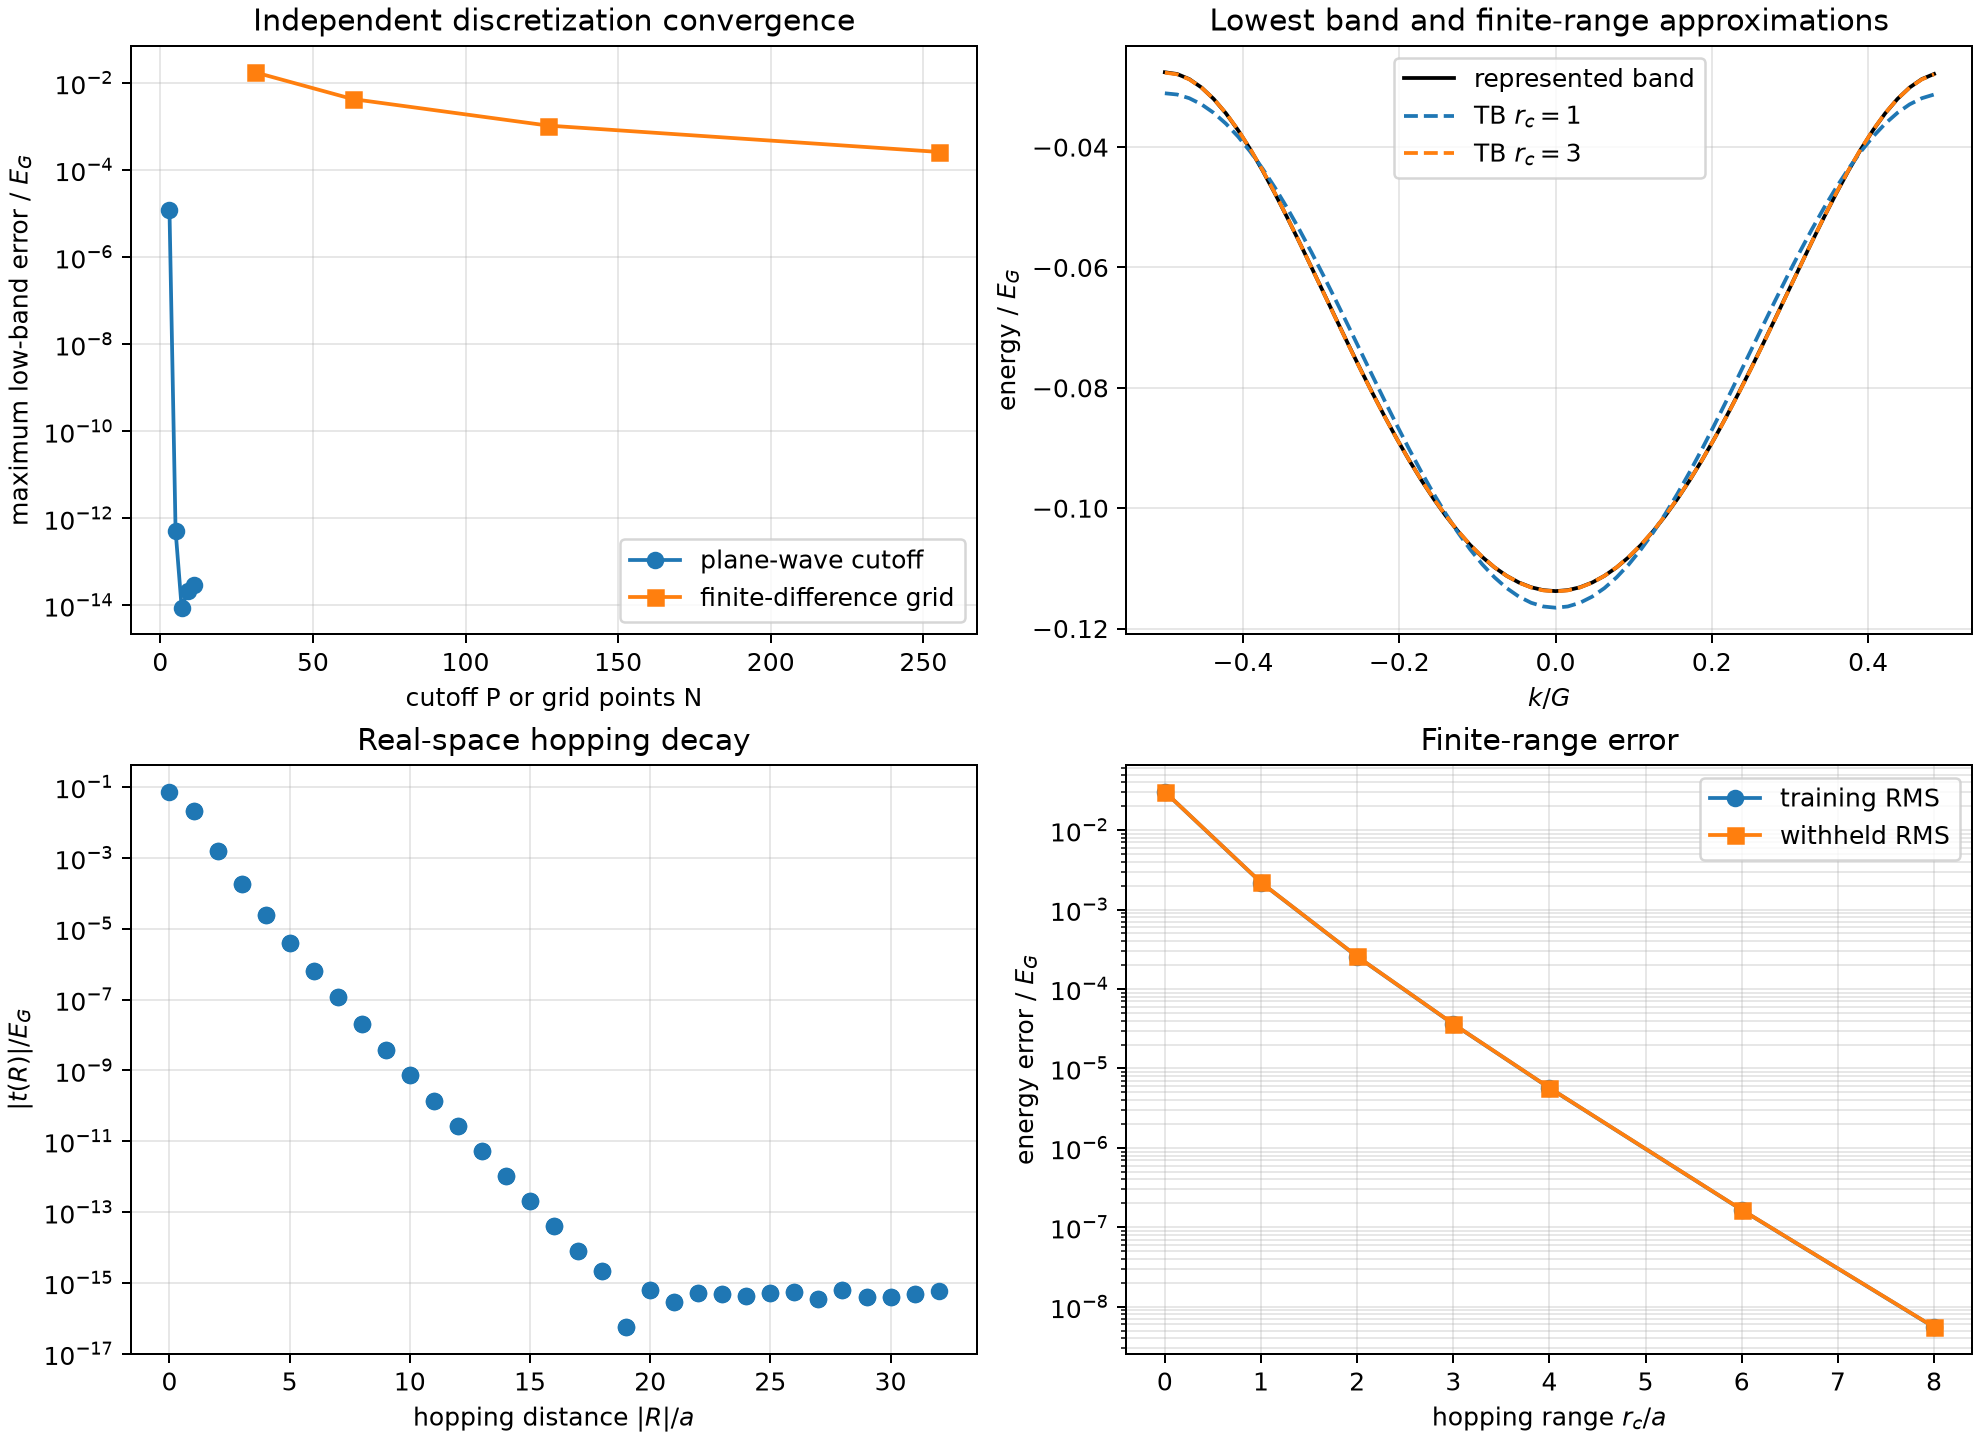
\includegraphics[
    width=\textwidth,
    height=0.82\textheight,
    keepaspectratio
  ]{../../../calculations/research-monograph/periodic-1d/summary.png}
  \caption{Isolated-band reduction at $V_0/E_G=0.5$. The independent
  plane-wave and finite-difference sequences converge at their expected rates
  (upper left). Increasing the hopping range improves the reconstructed lowest
  band (upper right) as the real-space coefficients decay (lower left).
  Training- and withheld-mesh root-mean-square errors remain nearly coincident
  across the range hierarchy (lower right).}
  \label{fig:periodic-1d-nominal}
\end{figure}

\subsection{Sensitivity and breakdown of scalar-band reduction}

The sensitivity study distinguishes robust structure from assumptions that hold
only in the baseline regime. Translation of the cosine changes the spectrum by
less than $8.9\times10^{-15}E_G$, and removal of the known constant shift restores
the baseline to the same tolerance. Every tested real potential preserves
spinless time-reversal energy symmetry within $2.0\times10^{-14}E_G$.

Cutoff adequacy depends on the claimed band range. The first eight $P=15$ bands
agree with the $P=21$ reference within $8.9\times10^{-15}E_G$ throughout the
amplitude sweep, whereas the corresponding $P=5$ error reaches
$1.25\times10^{-2}E_G$ at $V_0/E_G=4$. A cutoff verified for three low bands is
therefore not evidence for higher-band accuracy.

The free limit closes every tested isolation gap. At $V_0/E_G=0.5$, the minimum
adjacent gap falls from $4.92\times10^{-1}E_G$ for band 0 to
$1.20\times10^{-12}E_G$ for band 7. At the fixed range $r_c=3a$, the associated
withheld maximum error rises from $6.01\times10^{-5}E_G$ to
$2.02\times10^{-1}E_G$. Additional Fourier harmonics alter upper-band gaps by
orders of magnitude. Energy ordering alone is therefore not a stable
higher-band identity.

Random phase perturbations preserve projectors, transported frames, and closure
holonomy to binary64 precision. Route equivalence is lost, as expected, when the
fitting problem changes: nonuniform reciprocal weights give a coefficient
defect of $1.32\times10^{-5}$, while restricting the training region gives
$3.44\times10^{-4}$, compared with $5.2\times10^{-17}$ for the complete
uniform-mesh control. These coefficient route defects quantify the changed
fitting problems; they are not implementation residuals.
Figure~\ref{fig:periodic-1d-stress} collects the principal sensitivity results.

\begin{figure}[p]
  \centering
  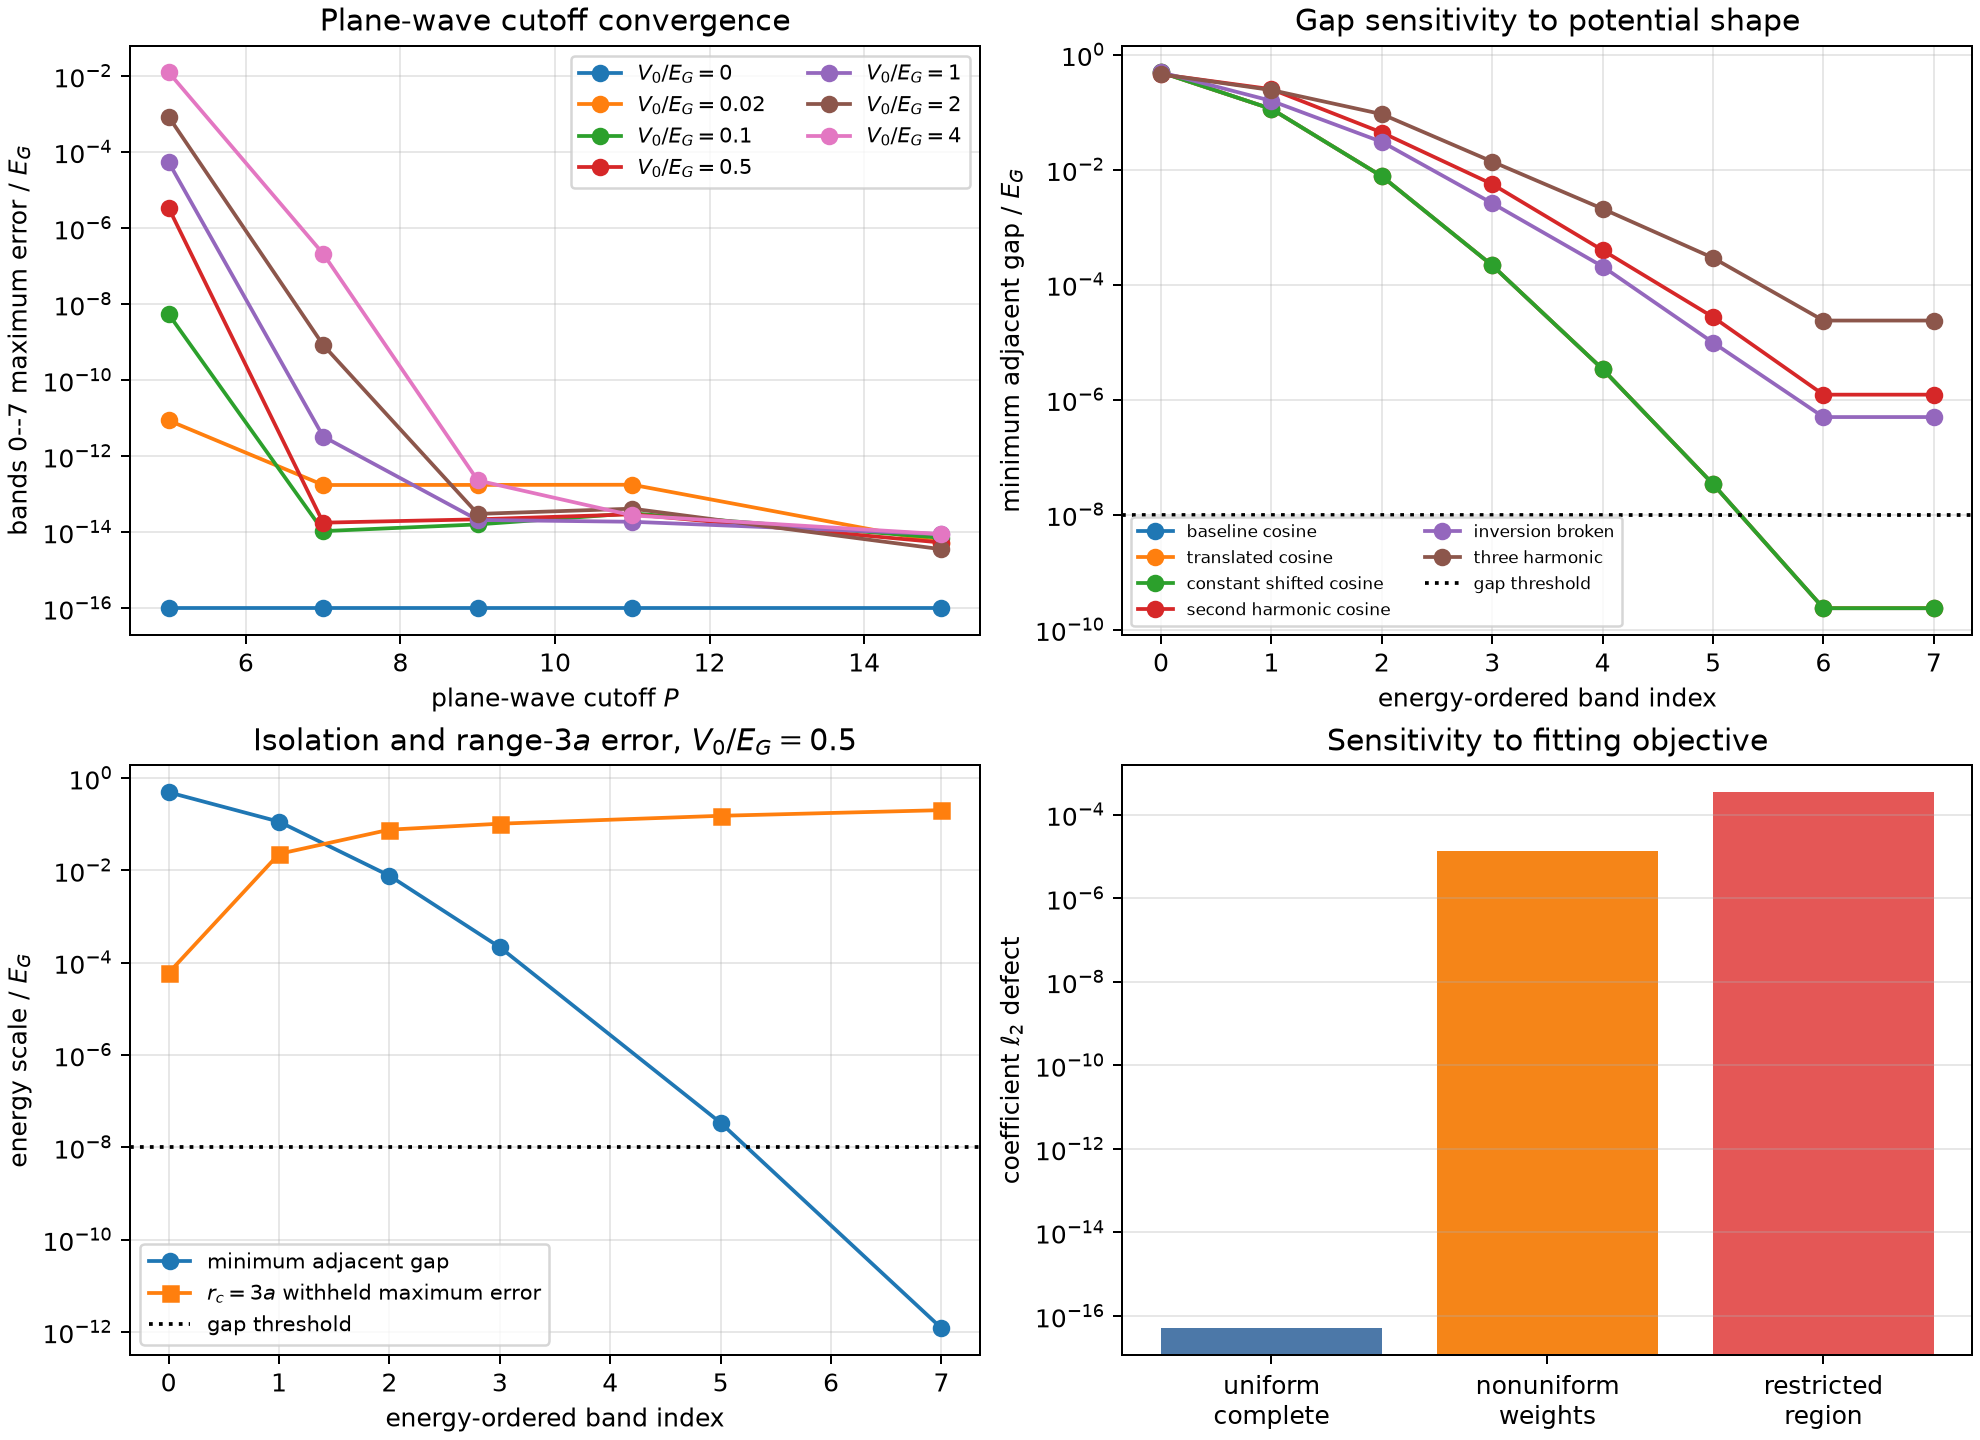
\includegraphics[
    width=\textwidth,
    height=0.82\textheight,
    keepaspectratio
  ]{../../../calculations/research-monograph/periodic-1d/stress-summary.png}
  \caption{Sensitivity of the reduction to cutoff, potential shape, band
  index, and fitting objective. Higher bands require larger plane-wave cutoffs
  (upper left), and their adjacent gaps depend strongly on the Fourier content
  of the potential (upper right). At fixed $V_0/E_G=0.5$, diminishing isolation
  accompanies increasing range-$3a$ error (lower left). Direct and mediated
  routes cease to coincide when their reciprocal weights or fitting domains
  differ (lower right).}
  \label{fig:periodic-1d-stress}
\end{figure}

\subsection{Composite-band remedy}

Bands 0--1 provide a well-conditioned composite baseline, while bands 2--3
provide a more difficult higher-band case. Table~\ref{tab:periodic-1d-composite}
shows the principal conditioning and reduction results. Both groups satisfy the
external-gap threshold, but the higher pair is much less isolated and has a
smaller minimum neighboring-overlap singular value.

\begin{table}[htbp]
  \centering
  \caption{Composite-band conditioning, centers, and range-$12a$ errors. Center
  defects compare the converged Wannier90 center set with the direct Wilson
  center set modulo one lattice period.}
  \label{tab:periodic-1d-composite}
  \begin{tabular}{lrrrr}
    \toprule
    Group & Ext. gap ($E_G$) & Min. $\sigma$ & Center defect ($a$) &
    Range-$12a$ error ($E_G$) \\
    \midrule
    Bands 0--1 & $1.14\times10^{-1}$ & 0.991696 &
    $2.16\times10^{-7}$ & $9.32\times10^{-4}$ \\
    Bands 2--3 & $2.16\times10^{-4}$ & 0.708327 &
    $2.63\times10^{-3}$ & $3.13\times10^{-2}$ \\
    \bottomrule
  \end{tabular}
\end{table}

Direct polar transport gives Wilson-loop eigenphases $\pm1.98562$ radians for
bands 0--1 and $\pm1.56593$ radians for bands 2--3. Under a controlled smooth
momentum-dependent $U(2)$ rotation, projector defects remain below
$5.1\times10^{-16}$, Wilson-phase set defects below $2.5\times10^{-15}$, and
represented eigenvalue defects below $7.6\times10^{-15}E_G$. Pointwise unitary
alignment recovers frames within $2.1\times10^{-15}$ and represented operators
within $6.9\times10^{-15}E_G$.

The complete block-hopping transforms reconstruct the reciprocal operators
within $3.3\times10^{-14}E_G$. Smooth polar frames yield monotonically improving
finite-range models. At $r_c=12a$, their withheld maximum errors are
$9.32\times10^{-4}E_G$ and $3.13\times10^{-2}E_G$. A deliberately rough
periodic gauge preserves the complete pointwise spectra but leaves errors of
$1.99\times10^{-1}E_G$ and $2.82\times10^{-1}E_G$. Thus gauge covariance of the
complete operator does not imply gauge invariance of a finite-range
truncation.

At $r_c=4a$, equal-weight direct matrix Fourier fitting and mediated block
truncation agree within $2.5\times10^{-15}$ in coefficient norm when they use
the same mesh, aligned frame, and model class. Figure~\ref{fig:periodic-1d-composite}
shows the conditioning, Wilson phases, hopping decay, and finite-range errors.

\begin{figure}[p]
  \centering
  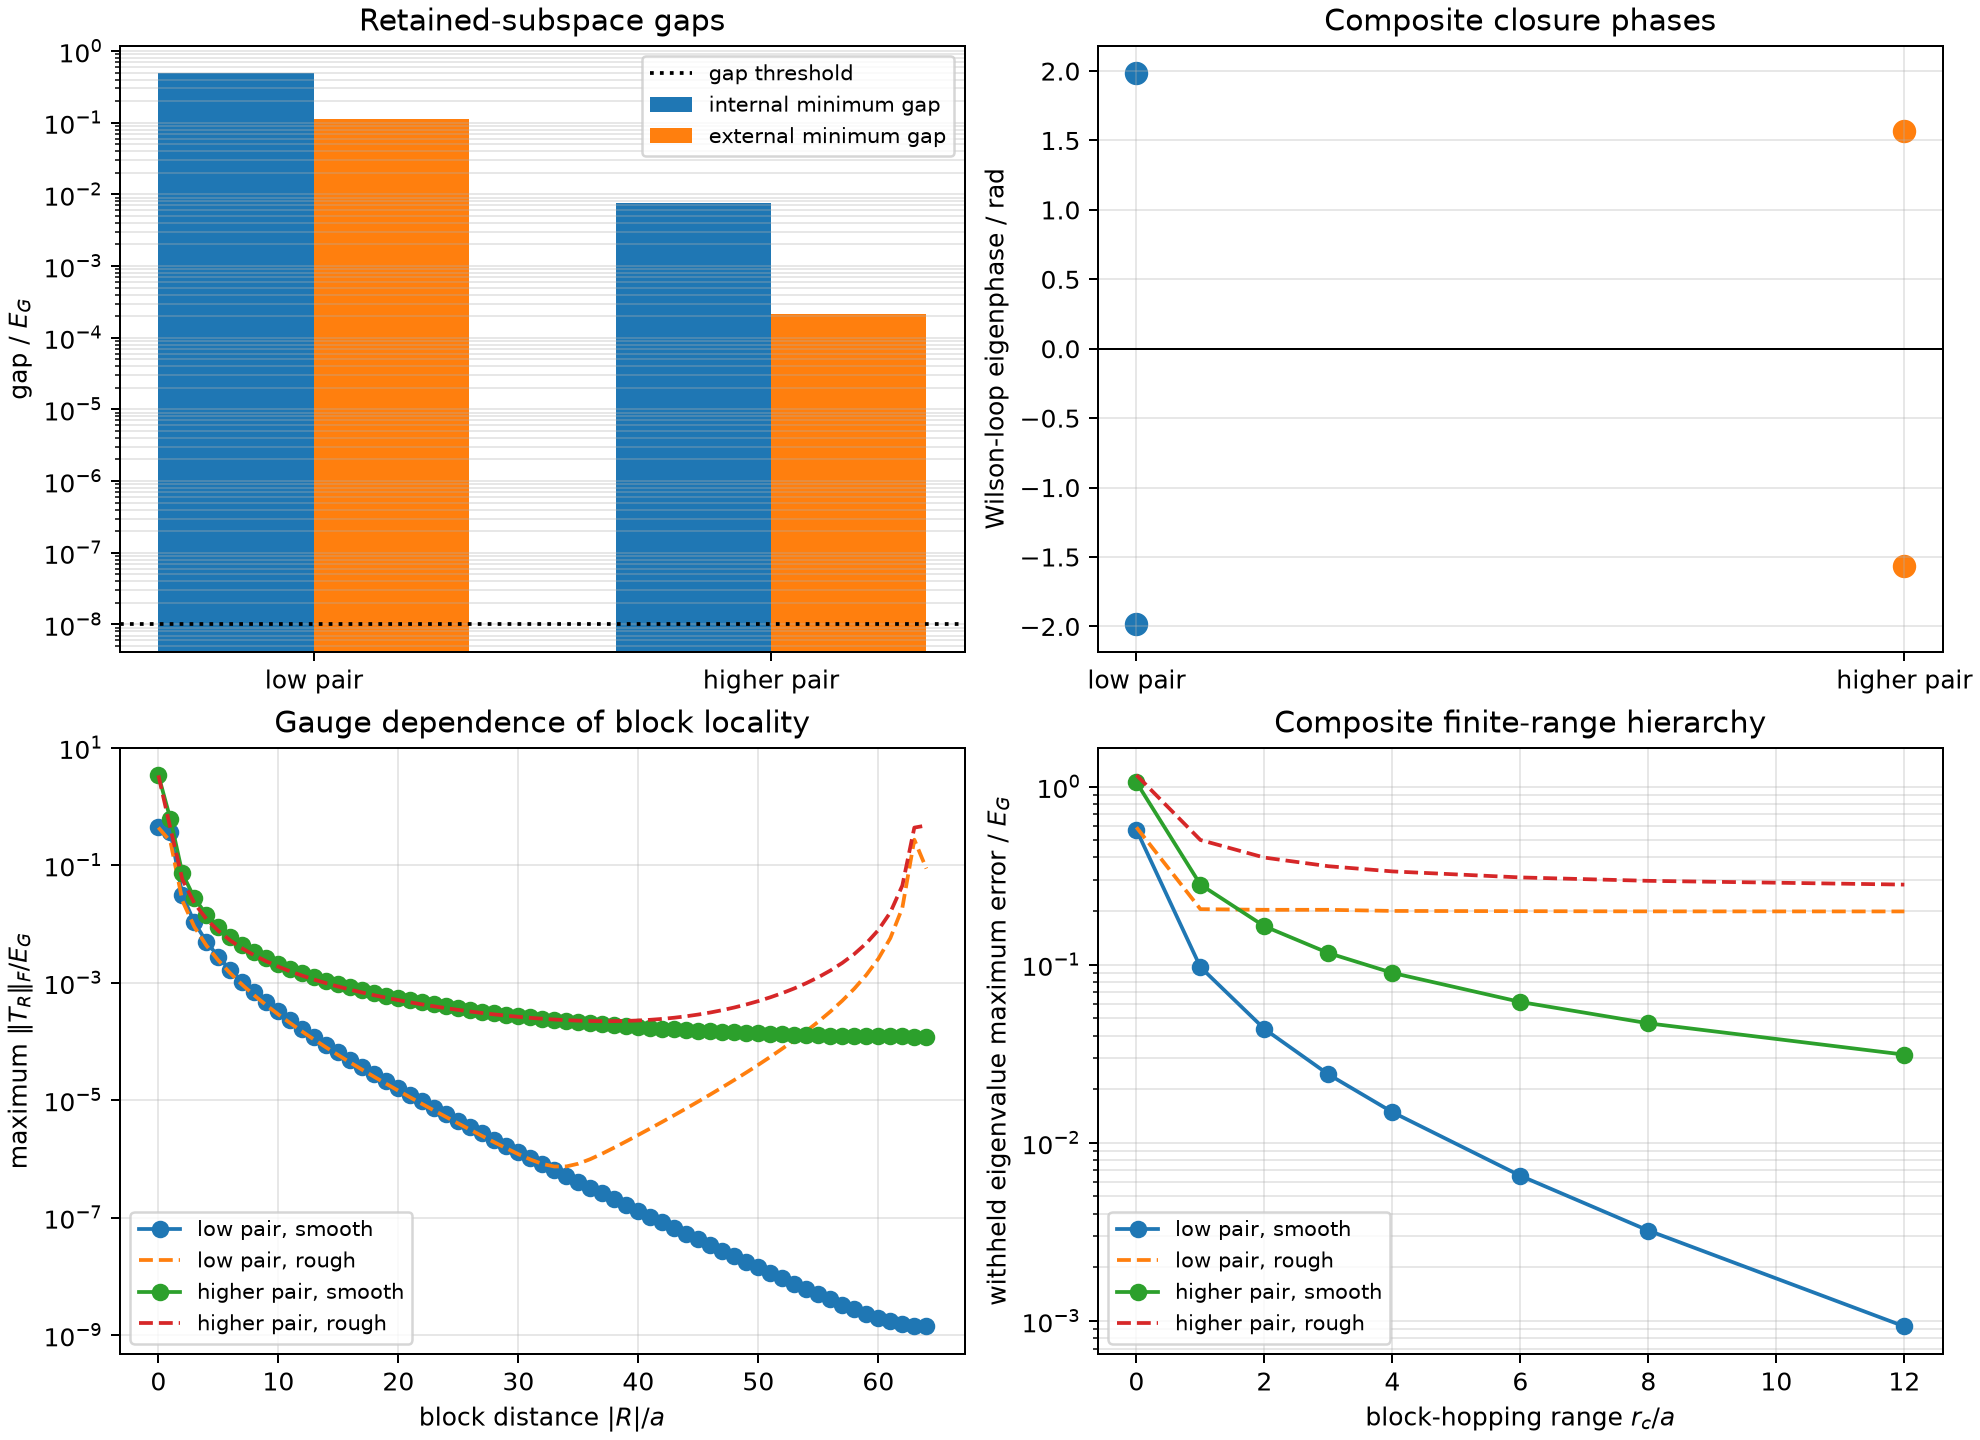
\includegraphics[
    width=\textwidth,
    height=0.82\textheight,
    keepaspectratio
  ]{../../../calculations/research-monograph/periodic-1d/composite-summary.png}
  \caption{Composite-band conditioning and finite-range reduction. Internal
  and external gaps distinguish the two retained band pairs (upper left), while
  Wilson-loop eigenphases determine their centers modulo a lattice period
  (upper right). Smooth polar frames produce more rapidly decaying hopping
  blocks (lower left) and smaller finite-range errors (lower right) than the
  spectrally equivalent rough gauges.}
  \label{fig:periodic-1d-composite}
\end{figure}

\subsection{Wannier90 localization}

The Wannier90 interface uses the same eigenvalues, band groups, overlap
matrices, reciprocal sewing, and auxiliary embedding as the direct calculation.
The strongly anisotropic mesh requires an extended reciprocal-shell
search to construct a neighbor list satisfying the three-dimensional B1
condition. With those data unchanged, unpreconditioned calculations remained
nonstationary at 500 iterations; increasing only the ceiling to 5000 iterations
also failed for the low pair. The spread decreased monotonically, and even the
smallest late-stage change remained above the prescribed tolerance. Relaxing
that tolerance would therefore have classified an evolving gauge as converged.

Wannier90 documents its real-space preconditioner for slow spread minimization
on fine reciprocal grids. Adding only \texttt{precond = true} while preserving
the parent, interface, objective, $10^{-12}$ tolerance, five-step window, and
5000-iteration ceiling changes the outcome. The low pair converges in 69
iterations and the higher pair in 4176. The total spreads are 0.337439093 and
3.673238490 cell$^2$, respectively.

The low-pair centers are $\{+0.316021,-0.316021\}a$ and agree with the direct
Wilson set within $2.16\times10^{-7}$ cell. Modulo lattice translations, the
higher-pair centers are $\{-0.246592,+0.246600\}a$, with a
$2.63\times10^{-3}$-cell discrepancy from the direct set. The discrepancy is reported without changing tolerances or relabelling
orbitals. It occurs in the group with the smaller external gap and poorer
overlap conditioning, but this calculation does not establish a unique causal
attribution.

The exported gauges are unitary within $1.9\times10^{-10}$ at their printed
precision. After pointwise alignment, the represented operators agree with the
direct construction within $4.9\times10^{-10}E_G$. At $r_c=12a$, the
Wannier90-gauge errors are $9.32\times10^{-4}E_G$ and
$3.09\times10^{-2}E_G$, close to the direct-polar values in
Table~\ref{tab:periodic-1d-composite}. The formatted \texttt{hr.dat} files add
separate maximum training eigenvalue discrepancies of approximately
$1.1\times10^{-5}E_G$ and $1.2\times10^{-4}E_G$.
Figure~\ref{fig:periodic-1d-wannier90-preconditioned} summarizes the converged
comparison.

\begin{figure}[p]
  \centering
  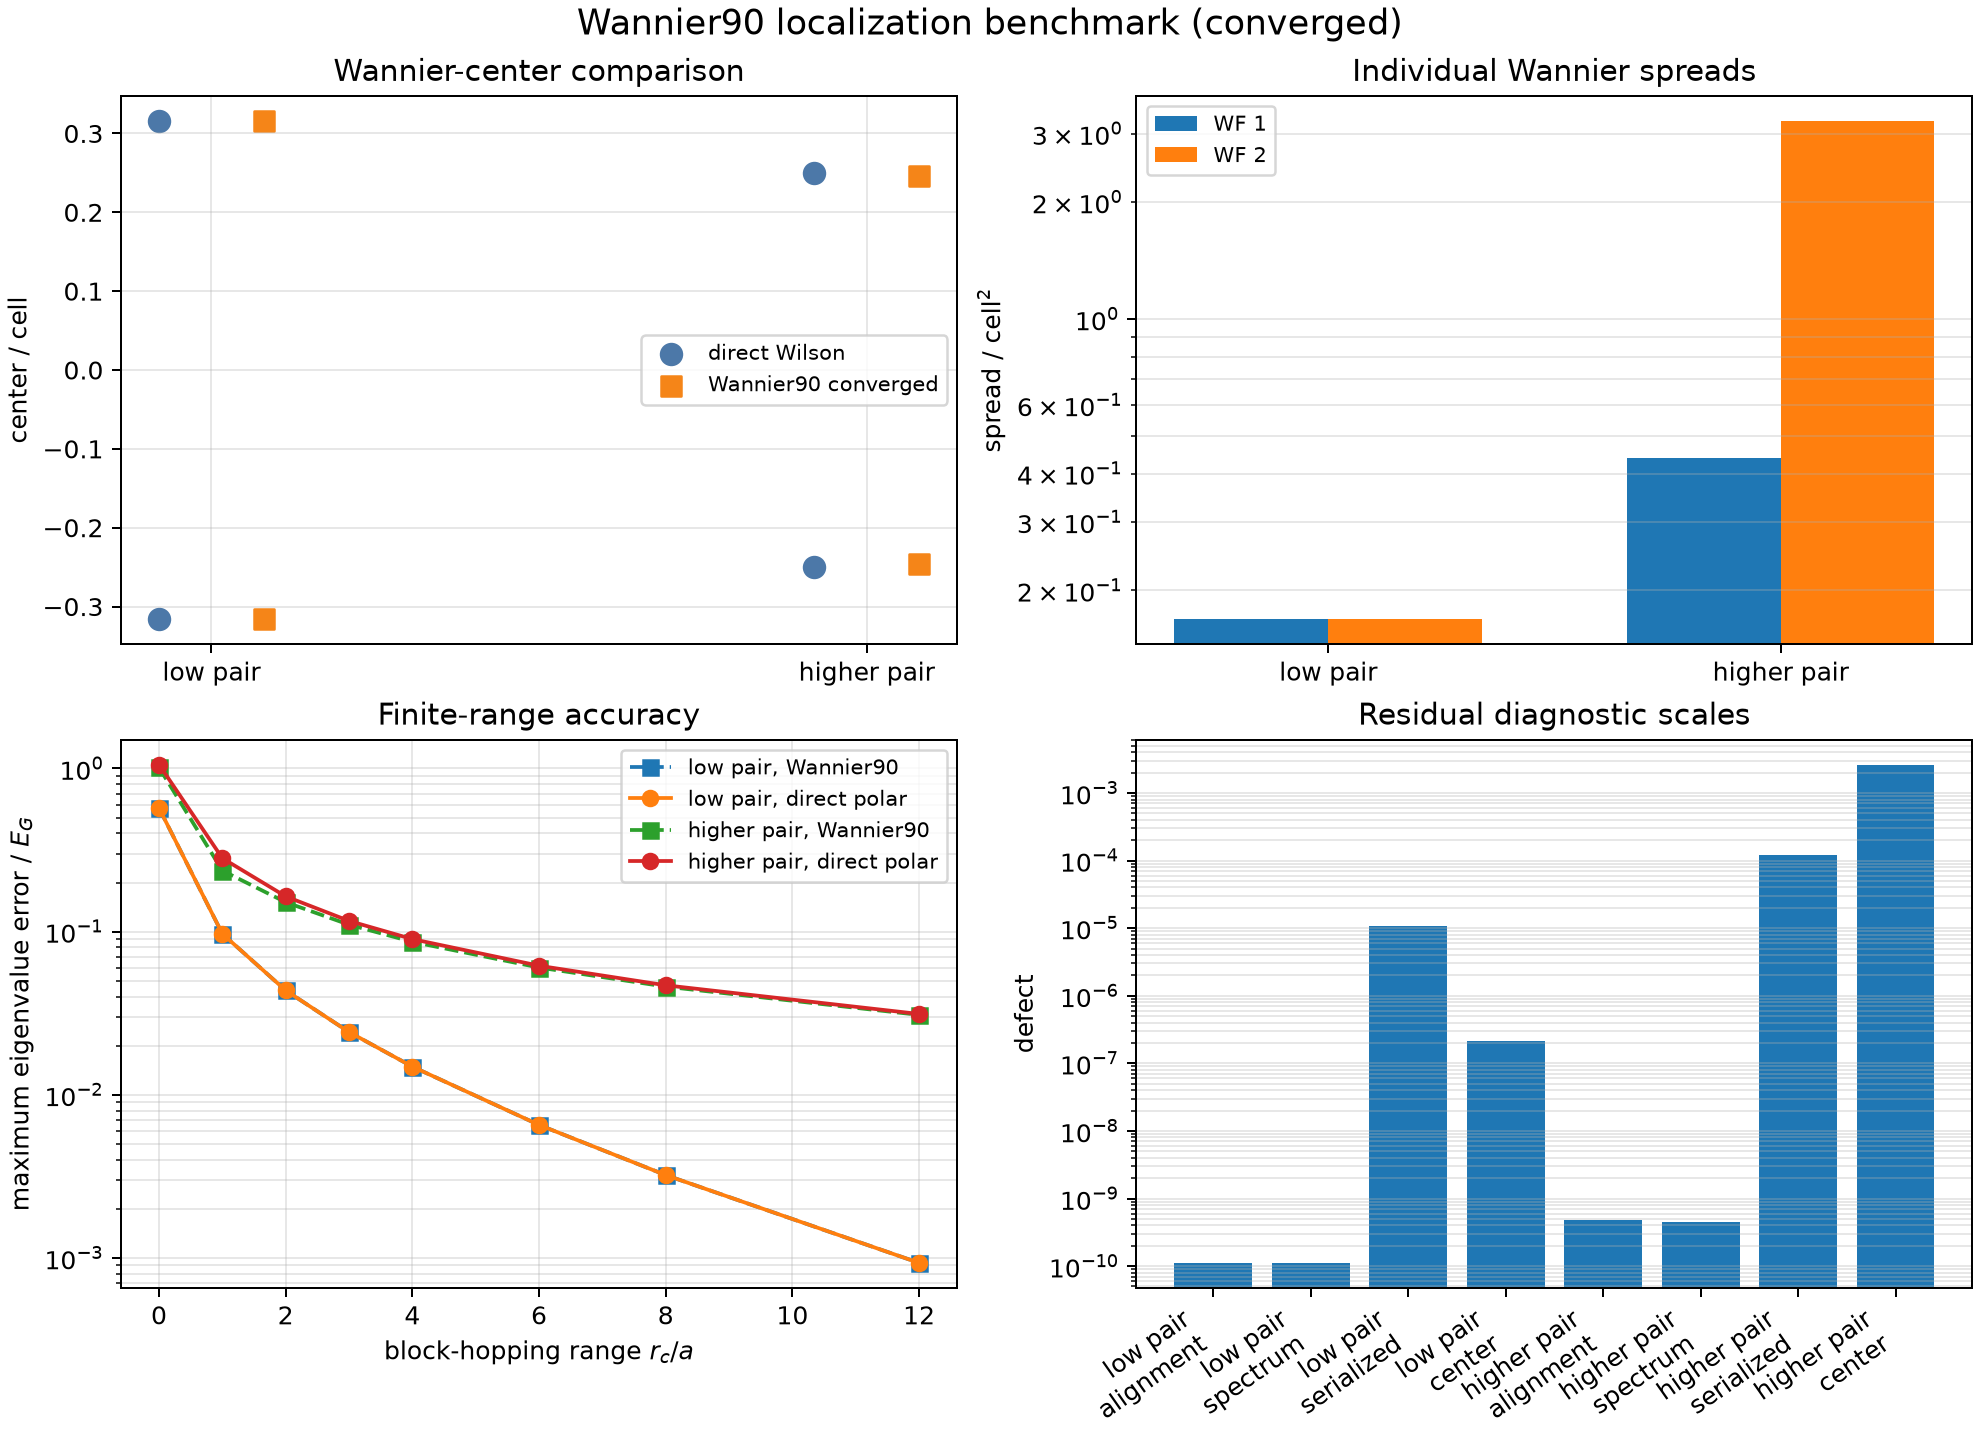
\includegraphics[
    width=\textwidth,
    height=0.82\textheight,
    keepaspectratio
  ]{../../../calculations/research-monograph/periodic-1d/wannier90-preconditioned-summary.png}
  \caption{Comparison between direct polar transport and converged,
  preconditioned Wannier90 localization. Centers are reduced modulo one lattice
  period (upper left), and individual Wannier spreads show the poorer locality
  of the higher pair (upper right). The two gauges give nearly identical
  finite-range errors after alignment (lower left); residual alignment,
  serialization, spectral, and center defects are shown separately (lower
  right).}
  \label{fig:periodic-1d-wannier90-preconditioned}
\end{figure}

\section{Discussion}

\subsection{Representation agreement requires an explicit map}

The parent comparison demonstrates why equality of eigenvalues is not a
sufficient operator comparison. The finite-difference and plane-wave matrices
act in different numerical spaces until the discrete Fourier map identifies a
common sector. Once that map is supplied, the low-mode discrepancy converges as
expected and can be attributed to the finite-difference stencil rather than to
an undefined subtraction. The same principle governs later pristine--doped and
cross-code comparisons: basis and state-space identification precede matrix
residuals.

\subsection{Band labels fail before composite subspaces do}

The sensitivity analysis shows a qualitative distinction between an
energy-ordered band and a retained subspace. As adjacent gaps collapse, scalar overlaps and
fixed-range models deteriorate even though a neighboring group can remain
transportable. Composite polar transport does not remove poor conditioning; it
makes that conditioning visible through singular values and external gaps while
preserving a gauge-covariant operator. This is the relevant analogue of a
multiorbital retained manifold.

\subsection{Localization controls truncation, not the complete spectrum}

Smooth and rough gauges produce complete operators with identical pointwise
spectra but markedly different block decay. Localization is therefore not a
cosmetic post-processing step when the final model is truncated. It selects the
coordinates in which a short-range approximation is attempted. The direct and
Wannier90 comparisons reinforce the same conclusion: raw hopping blocks cannot
be compared across gauges, while aligned complete operators can.

\subsection{Route equivalence has precise hypotheses}

Agreement between direct fitting and mediated truncation is exact only when the
two calculations implement the same finite Fourier projection. The controlled
weight and training-domain changes break those hypotheses and produce nonzero
route defects without indicating a software failure. In a material
calculation, the route defect must therefore be interpreted together with the
fitting measure, model constraints, gauge, and comparison domain.

\subsection{Implications for multiband reductions}

This calculation verifies the middle of the intended reduction chain: retained
Bloch information can be transported into localized coordinates, reconstructed
as a complete lattice operator, and truncated with separately measured error.
It also supplies explicit breakdown cases for weak isolation, unstable scalar
labels, rough gauges, and mismatched fitting objectives. These observations
define concrete diagnostics for a subsequent silicon calculation. The present
benchmark does not test a
Kohn--Sham parent, a three-dimensional crystal, pristine--doped alignment, an
impurity operator, multivalley structure, spin--orbit coupling, or a continuum
effective-mass reduction.

\section{Limitations and scope}

The results establish numerical behavior only for the specified cosine parent.
Several limitations remain:
\begin{itemize}
    \item The transverse Wannier90 embedding and identity trial projections are
          synthetic conventions rather than material-derived orbitals.
    \item The study contains no reciprocal-mesh convergence analysis of the
          final Wannier90 centers across alternative projection choices.
    \item The higher pair is only weakly separated from excluded bands, and its
          center discrepancy is not assigned to one error source.
    \item No hopping range is selected for a physical use because no
          application-specific accuracy threshold is specified.
    \item The calculations do not establish scientific validation,
          uncertainty quantification, or transferability to silicon.
\end{itemize}
The successful convergence of two numerical routes does not promote the cosine
model into a semiconductor result. Likewise, the failed intermediate Wannier90
calculations diagnose optimizer behavior for this interface; they do not
contradict the direct composite
construction.

\section{Conclusions}

The one-dimensional cosine lattice provides a controlled test of the complete
Bloch-to-lattice reduction rather than of any one eigensolver or localization
algorithm. Independent parent discretizations converge toward a common
low-mode operator, and the isolated lowest band admits a rapidly convergent hopping
expansion. Direct Fourier fitting and localized-operator truncation agree when
they implement the same projection and diverge when their weights or fitting
domains differ.

The multiband calculations identify the principal boundary of the scalar
construction. Near small adjacent gaps, energy-ordered labels become poorly
conditioned before the composite subspace is lost. Composite transport restores
a coherent operator description, but finite-range accuracy remains dependent on
the gauge in which truncation is performed. The converged Wannier90 comparison
reproduces the aligned operators and low-pair centers while preserving a finite
higher-pair center discrepancy. These results support the use of explicit
subspace, alignment, localization, and truncation diagnostics in more complex
periodic reductions; they do not by themselves establish accuracy for a
semiconductor Hamiltonian.

\section{Computational reproducibility}

Inputs, calculation programs, deterministic verification scripts, numerical
results, figures, and SHA-256 checksums are available under
\path{calculations/research-monograph/periodic-1d/}. Separate records distinguish
the isolated-band calculation, sensitivity analysis, composite-band
calculation, unconverged Wannier90 iterations, and converged preconditioned
calculation. Large native Wannier90 artifacts remain outside the repository and
are identified by file size and SHA-256 digest in the execution metadata.

The reports \texttt{report.md} and \texttt{composite-report.md} provide exact
reproduction commands and additional numerical detail. The verification scripts
test the stated numerical contracts; they do not constitute material validation
or evidence of transferability to silicon.
